\documentclass[12pt]{article}
\usepackage{amsmath,amssymb,amsthm}
\usepackage{graphicx}
\usepackage{fullpage}
\usepackage[innercaption]{sidecap}
\newcommand{\estart}
{
\renewcommand{\labelenumi}{(\alph{enumi})}
\vspace{-0.5\baselineskip}
\begin{enumerate}
}

\newcommand{\eend}
{
\end{enumerate}
\renewcommand{\labelenumi}{(\arabic{enumi})}
}

\usepackage{rotating}


\usepackage[absolute]{textpos}
\setlength{\TPHorizModule}{1mm}
\setlength{\TPVertModule}{1mm}

\begin{document}

\pagestyle{empty}

\section*{Summary: Polynomial Interpolation (Chapter 5)}

\begin{textblock}{170}(10,260)
\noindent \textsf{{\small Intro Scientific Computing and Data Analysis, M. H. Holmes, 2nd ed (version: \today)}}
\end{textblock}

\bigskip\bigskip\noindent
\textbf{Interpolation Points:} $(x_1,y_1),  (x_2,y_2), \cdots , (x_{n+1},y_{n+1})$, where $x_1 < x_2 < \cdots < x_{n+1}$

\bigskip\bigskip\bigskip\noindent
\textbf{Global Polynomial Interpolation}
\[
p_n(x)= \ell(x) { \sum_{i=1}^{n+1} \frac{ w_iy_i}{x-x_i}  } 
\tag{5.8}
\]
\hspace{0.1in} where
\[
\ell(x) =(x-x_1)(x-x_2) \cdots  (x-x_{n+1}) =\prod_{j=1}^{n+1} (x-x_j)
\]
\hspace{0.1in} and
\[
w_i=\frac{1}{(x_i-x_1)(x_i-x_2) \cdots (x_i-x_{i-1})(x_i-x_{i+1})\cdots (x_i-x_{n+1})} = \Bigg ( \prod_{\substack{j=1 \\ j\neq i}}^{n+1} (x_i-x_j) \Bigg )^{-1}
\]

\bigskip\bigskip\noindent
Chebyshev interpolation: $x_i =  \frac{1}{2} \! \left[ a+b+(b-a)z_i \right ]$, where $z_i = \cos \! \left ( \frac{2i-1}{2(n+1)} \pi \right )$


\bigskip\bigskip\bigskip\bigskip\noindent
\textbf{Piecewise Linear Interpolation}
\[
g(x)=\sum_{i=1}^{n+1}y_i G_i (x)
\tag{5.15}
\]
\hspace{1in} where
\[
G_i (x)=
\begin{cases}
\,\, 0 & \text{if \,\,}  x \leq x_{i-1}, \medskip \\ 
{\displaystyle  \frac{x-x_{i-1}}{x_i-x_{i-1}} } & \text{if \,\,} x_{i-1} \leq x \leq x_i,  \medskip  \\
{\displaystyle    \frac{x-x_{i+1}}{x_i-x_{i+1}} }  & \text{if \,\,} x_{i} \leq x \leq x_{i+1},  \medskip \\
\,\, 0 & \text{if \,\,} x_{i+1} \leq x 
\label{eq:4.Gi}
\end{cases}
\]
Equally spaced nodes:
\[
G_i (x)= G \! \left( \frac{x-x_i}{h} \!  \right )
\]
\hspace{1in} and
\[
G (x)=
\begin{cases}
\,\, 1-|x| & \text{if \,\,}  |x| \leq 1, \\[0.2em]
\,\, 0 & \text{if \,\,} 1 \leq |x| 
\label{eq:inter.G}
\end{cases}
\]

\newpage\noindent
\textbf{Piecewise Cubic Interpolation (equally spaced)}
\[
s(x)=\sum_{i=0}^{n+2}a_i B_i (x)
\tag{5.27}
\]
\hspace{1in} where
\[
B_{i}(x)= B \!\! \left ( \frac{x-x_i}{h}\right )
\tag{5.23}
\]
\hspace{1in} and
\[
B (x)=
\begin{cases}
{\,  \frac{2}{3}  - x^2 \! \left (1- \frac{1}{2} |x| \right ) } &\text{ if \,\,}   |x| \leq 1,  \\[0.4em]
{ \,  \frac{1}{6}(2- |x|)^3 } & \text{ if \,\,} 1 \leq |x| \leq 2, \\[0.4em]
 \, 0 & \text{ if \,\,} 2 \le |x|
\end{cases}
\]

\bigskip\noindent
Natural Spline:  $s''(x_1)=0$ and $s''(x_{n+1})=0$\\[0.2em]
\noindent
Clamped Spline:  $s'(x_1)=y_1'$ and $s'(x_{n+1})=y_{n+1}'$\\[0.2em]
\noindent
Not-a-Knot Spline (for $n >2$):  $s_1'''(x_2)=s_2'''(x_2)$ and $s_{n-1}'''(x_{n})=s_n'''(x_{n})$\\


\begin{table}[h]
\centering
\renewcommand\arraystretch{2}
\renewcommand\tabcolsep{6pt}
\begin{tabular}{c|c|c|c|c} 
 & {\normalsize $x_{i-1}$} & {\normalsize $x_i$} & {\normalsize $x_{i+1}$} & {\normalsize $x_{j}$} for {\normalsize $j \ne  i , i\pm1$} \\ \hline
{\normalsize $B_i$}  & {\large $\frac{1}{6}$} & {\large $\frac{2}{3}$}& {\large $\frac{1}{6}$} & {\normalsize $0$}\\ \hline
{\normalsize $B_i^{\prime}$}  & {\large $\frac{1}{2h}$} & {\normalsize $0$}&  {\large $- \frac{1}{2h}$} & {\normalsize $0$}\\ \hline
{\normalsize $B_i^{\prime \prime}$}  &  $1/h^2$ & $-2/h^2$ & $1/h^2$ & {\normalsize $0$} \\ 
\end{tabular}
\caption{Values of $B_i(x)$ at the nodes.}
\end{table}

\begin{figure}[b]
\centering
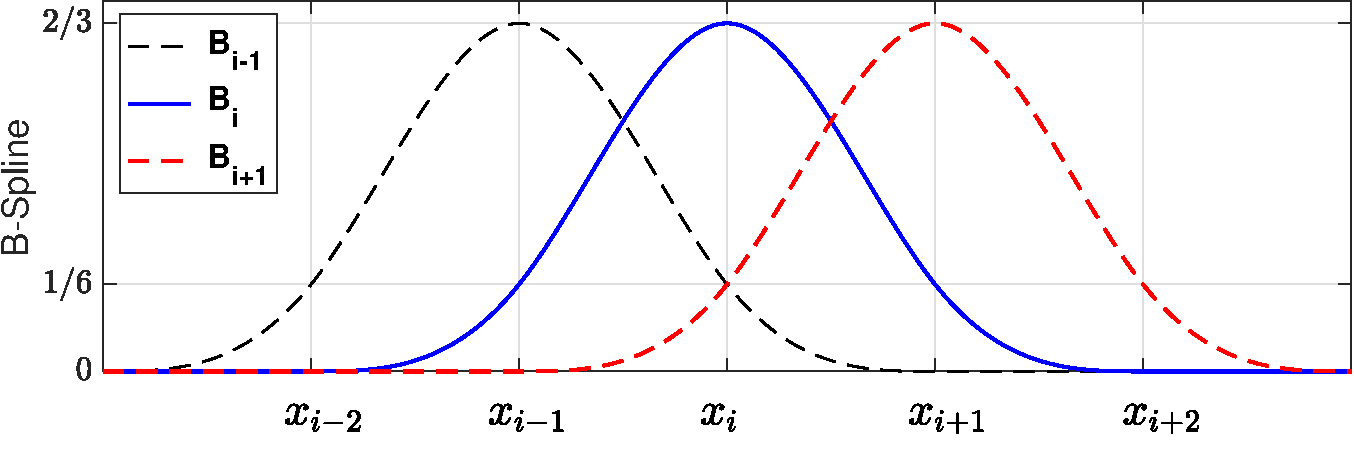
\includegraphics[width=5.2in]{bspline.pdf}
\caption{Plot of the cubic B-splines $B_{i-1}(x)$, $B_i(x)$, and  $B_{i+1}(x)$. }
\label{fig:inter.b}
\end{figure}

















 \end{document}
 

